\documentclass[14pt]{article}
\usepackage[utf8]{inputenc}
\usepackage[T2A]{fontenc}
\usepackage[russian]{babel}
\usepackage{amsmath, amssymb}
\usepackage{geometry}
\usepackage{graphicx}
\usepackage{xcolor}
\usepackage{hyperref}
\usepackage{tasks}
\usepackage{tcolorbox}
\tcbuselibrary{skins, breakable, theorems}
\usepackage{fancyhdr}
\usepackage{lastpage}
\usepackage{enumitem}
\usepackage{paracol} % Для многоколоночности
\usepackage{ifthen}
\usepackage{needspace}

% Определение команд для тангенса и котангенса (русский стиль)
\newcommand{\tg}{\operatorname{tg}}
\newcommand{\ctg}{\operatorname{ctg}}

% Настройка геометрии для более компактного вида (как в мобильных приложениях)
\geometry{a4paper, left=10mm, right=10mm, top=20mm, bottom=20mm, headheight=15pt}

% Цветовая палитра (более современные и мягкие цвета)
\definecolor{primary}{RGB}{52, 152, 219}       % Ярко-синий
\definecolor{secondary}{RGB}{46, 204, 113}     % Зеленый
\definecolor{accent}{RGB}{155, 89, 182}        % Фиолетовый
\definecolor{lightbg}{RGB}{248, 249, 250}      % Светло-серый фон
\definecolor{taskborder}{RGB}{230, 230, 230}   % Цвет границы задач
\definecolor{optionbg}{RGB}{240, 242, 245}     % Фон для вариантов ответа

% Основной фон страницы
\pagecolor{lightbg}

% Настройка гиперссылок
\hypersetup{
    colorlinks=true,
    linkcolor=primary,
    urlcolor=primary,
}

% Колонтитулы (более стильные)
\pagestyle{fancy}
\fancyhf{}
\fancyhead[L]{\textcolor{primary}{\textbf{MathCore | MOCK Test-6}}}
\fancyhead[R]{\textcolor{secondary}{Abdunazarov M.X.}}
\fancyfoot[L]{\href{https://t.me/Math_Core_Dtm_MS_Att}{\textcolor{primary}{MathCore}}}
\fancyfoot[R]{\href{https://t.me/Abd_mardon}{\textcolor{secondary}{@Abd\_mardon}}}
\fancyfoot[C]{\textcolor{gray}{\thepage/\pageref{LastPage}}}
\renewcommand{\headrulewidth}{0.5pt}
\renewcommand{\headrule}{\hbox to\headwidth{\color{primary}\leaders\hrule height \headrulewidth\hfill}}
\renewcommand{\footrulewidth}{0.5pt}
\renewcommand{\footrule}{\hbox to\headwidth{\color{secondary}\leaders\hrule height \footrulewidth\hfill}}

% Титульная страница (улучшенная)
\title{\Huge \textbf{\textcolor{primary}{MOCK Test-6}}}
\author{\textcolor{secondary}{Abdunazarov M.X.}}
\date{}

% Стиль для карточки вопроса
\newtcolorbox{questionbox}[2][]{
    enhanced,
    breakable,
    colback=white,
    colframe=primary,
    coltitle=white,
    fonttitle=\bfseries\large,
    title={Задача \hfill \textcolor{white}{#2}},
    attach boxed title to top left={xshift=5mm, yshift=-2mm},
    boxed title style={size=small, colback=primary, sharp corners},
    sharp corners,
    boxrule=0.5pt,
    left=5mm,
    right=5mm,
    top=5mm,
    bottom=5mm,
    drop fuzzy shadow,
    #1
}

% Стиль для вариантов ответов (как кнопки)
\newlist{options}{enumerate}{1}
\setlist[options]{
    label=\textbf{\Alph*)},
    leftmargin=*,
    itemsep=2pt,
    topsep=5pt,
    before={\vspace{2mm}\begin{tcolorbox}[
        colback=optionbg,
        colframe=white,
        sharp corners,
        boxrule=0pt,
        left=2mm,
        right=2mm,
        top=2mm,
        bottom=2mm,
    ]},
    after={\end{tcolorbox}\vspace{2mm}},
}

% Для рисунков (центрирование и тень)
\newcommand{\questionimage}[2][0.5\linewidth]{%
    \begin{center}
        \includegraphics[width=#1]{#2}
    \end{center}
}

% Для удобства: команда вставки вопроса с рисунком
\newcommand{\questionitem}[4]{%
    \needspace{5cm} % Предотвращает разрыв вопроса
    \begin{questionbox}{#1}
        #2
        \ifx&#3&% Если рисунок не пустой
        \else
            \questionimage{#3}
        \fi
        \begin{options}
            #4
        \end{options}
    \end{questionbox}
}

\begin{document}

% Титульная страница
\maketitle
\begin{center}
    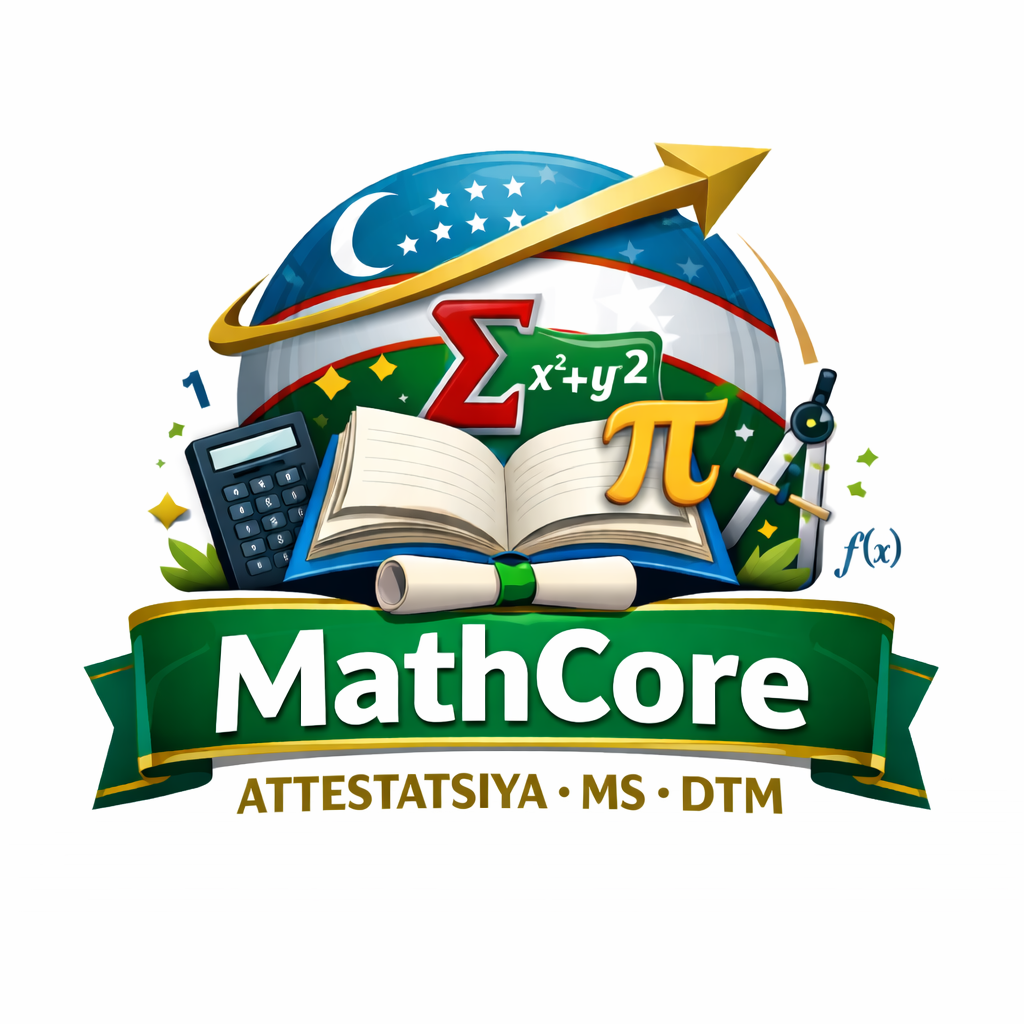
\includegraphics[width=0.2\textwidth]{logo.png} \\[5mm]
    \textcolor{gray}{\small Telegram: \href{https://t.me/Math_Core_Dtm_MS_Att}{@Math\_Core\_Dtm\_MS\_Att}}
\end{center}
\vspace{5mm}
% Задача 1
\begin{questionbox}{1}
    Найдите количество чётных натуральных делителей числа 2016.
    \begin{options}
        \item 16
        \item 30
        \item 36
        \item определить невозможно
    \end{options}
\end{questionbox}



% Задача 2
\begin{questionbox}{2}
    Вычислите: \( (((-2)^3)^4)^5 + ((-2^4)^3)^5 = ? \)
    \begin{options}
        \item \(-2^{61}\)
        \item \(-2^{60}\)
        \item \(0\)
        \item \(2^{61}\)
    \end{options}
\end{questionbox}



% Задача 3
\begin{questionbox}{3}
    Найдите остаток от деления значения выражения \(1^3+2^3+\ldots+100^3\) на 3.
    \begin{options}
        \item 0
        \item 1
        \item 2
        \item определить невозможно
    \end{options}
\end{questionbox}



% Задача 4
\begin{questionbox}{4}
    Если для натуральных чисел \(x\) и \(y\) выполняется соотношение \(\frac{(24!)^2 - (23!)^2}{5^x} = y\), найдите наибольшее возможное значение \(x\).
    \begin{options}
        \item 10
        \item 9
        \item 8
        \item 7
    \end{options}
\end{questionbox}



% Задача 5
\begin{questionbox}{5}
    Решите уравнение: \(\frac{x}{1-\frac{1}{2}} + \frac{x}{1-\frac{1}{3}} + \frac{x}{1-\frac{1}{4}} = 29\).
    \begin{options}
        \item 6
        \item 5
        \item 4
        \item 3
    \end{options}
\end{questionbox}



% Задача 6
\begin{questionbox}{6}
    Сколько цифр в произведении \(64^{15} \cdot 25^{46} \cdot 40^{3}\)?
    \begin{options}
        \item 67
        \item 92
        \item 94
        \item 97
    \end{options}
\end{questionbox}



% Задача 7
\begin{questionbox}{7}
    На отрезке \([200; 1000]\) сколько натуральных чисел при делении на 2, 3, 5 и 7 дают остаток 1?
    \begin{options}
        \item 4
        \item 3
        \item 2
        \item 1
    \end{options}
\end{questionbox}



% Задача 8
\begin{questionbox}{8}
    Для функции \(f(x) = \begin{cases} 3x - a, & x < -2 \\ x^2 + 3, & x \geq -2 \end{cases}\) выполняется равенство \(f(1) + f(-3) = 13\). Найдите \(a\).
    \begin{options}
        \item \(-22\)
        \item \(-20\)
        \item \(-18\)
        \item \(-16\)
    \end{options}
\end{questionbox}



% Задача 9
\begin{questionbox}{9}
    Если \(x^2 - 4x + 3 = 0\), то \(x^2 + \frac{9}{x^2} = ?\)
    \begin{options}
        \item 10
        \item 11
        \item 12
        \item 13
    \end{options}
\end{questionbox}



% Задача 10
\begin{questionbox}{10}
    Если \(x - y = y - z = 5\), то \(x^2 - 2y^2 + z^2 = ?\)
    \begin{options}
        \item 30
        \item 40
        \item 50
        \item 60
    \end{options}
\end{questionbox}



% Задача 11
\begin{questionbox}{11}
    Для положительных чисел a, b, c найдите наибольшее значение выражения \(\frac{a+4b+9c}{\sqrt{a^2+b^2+c^2}}\).
    \begin{options}
        \item \(\frac{14}{\sqrt{3}}\)
        \item \(7\sqrt{2}\)
        \item 14
        \item \(4\sqrt{3}\)
    \end{options}
\end{questionbox}



% Задача 12
\begin{questionbox}{12}
    Решите уравнение: \(\sqrt{5+ \sqrt{10}}  = x \cdot \left(\sqrt{5+ \sqrt{15}}  + \sqrt{5- \sqrt{15}}\right)\).
    \begin{options}
        \item \(\frac{1}{\sqrt{2}}\)
        \item \(\frac{1}{2}\)
        \item 2
        \item \(\sqrt{2}\)
    \end{options}
\end{questionbox}



% Задача 13
\begin{questionbox}{13}
    Если \(f(3x + 2) = \arcsin(6x - 1)\), то \(f\left(\frac{11}{4}\right) - f(2) = ?\)
    \begin{options}
        \item \(-\frac{\pi}{3}\)
        \item \(\frac{2\pi}{3}\)
        \item \(\frac{3\pi}{5}\)
        \item \(-\frac{\pi}{6}\)
    \end{options}
\end{questionbox}



% Задача 14
\begin{questionbox}{14}
    Для действительных чисел a, b, c дана система:
    \[
    \begin{cases} \frac{a \cdot b}{a+b} = \frac{3}{2} \\ \frac{b \cdot c}{b+c} = \frac{3}{2} \\ \frac{a \cdot c}{a+c} = \frac{3}{4} \end{cases}
    \]
    Найдите значение \(\frac{1}{a} + \frac{1}{b} + \frac{1}{c}\).
    \begin{options}
        \item \(\frac{3}{2}\)
        \item \(\frac{5}{2}\)
        \item \(\frac{5}{4}\)
        \item \(\frac{4}{3}\)
    \end{options}
\end{questionbox}



% Задача 15
\begin{questionbox}{15}
    Дано: \(\begin{cases} x = 1 + 3 + 5 + \dots + 99 \\ y = 2 + 4 + 6 + \dots + 100 \end{cases}\). Найдите \(\frac{x+y}{|x-y|} = ?\)
    \begin{options}
        \item \(\frac{101}{2}\)
        \item 101
        \item 111
        \item 102
    \end{options}
\end{questionbox}



% Задача 16
\begin{questionbox}{16}
    Сколько натуральных решений имеет неравенство \((4x - 12)^3 \leq (x + 15)^3\)?
    \begin{options}
        \item 11
        \item 10
        \item 9
        \item 8
    \end{options}
\end{questionbox}



% Задача 17
\begin{questionbox}{17}
    Если значение выражения \(\left[\frac{1}{4} : \left(\frac{1}{6} - \frac{1}{5}\right) + \frac{1}{4} : \frac{1}{3}\right] : \frac{3}{4} + x\) является целым положительным числом, найдите наименьшее значение \(x\).
    \begin{options}
        \item 9
        \item 10
        \item 11
        \item 12
    \end{options}
\end{questionbox}



% Задача 18
\begin{questionbox}{18}
    Дан отрезок \(AB\) с концами в точках \(A(7; -3)\) и \(B(19; -11)\). Найдите сумму координат точки \(C(a; b)\), которая делит отрезок \(AB\) в отношении \(\frac{AC}{BC} = 3\).
    \begin{options}
        \item 3
        \item 5
        \item 7
        \item 8
    \end{options}
\end{questionbox}



% Задача 19
\begin{questionbox}{19}
    Сторона основания правильной четырехугольной призмы равна 15, высота равна 20. Найдите кратчайшее расстояние от стороны основания до диагонали призмы, не пересекающей эту сторону.
    \begin{options}
        \item 16
        \item 15
        \item 14
        \item 12
    \end{options}
\end{questionbox}



% Задача 20
\begin{questionbox}{20}
    Упростите выражение: \(\cos^2 230^\circ \cdot (1 + \operatorname{ctg}220^\circ) + \sin^2 310^\circ \cdot (1 - \operatorname{ctg} 50^\circ)\).
    \begin{options}
        \item 2
        \item 1
        \item 0
        \item 3
    \end{options}
\end{questionbox}



% Задача 21
\begin{questionbox}{21}
    Решите уравнение: \(\frac{3ab+1}{a} x = \frac{3ab}{a+1} + \frac{(2a+1)x}{a(a+1)^2} + \frac{a^2}{(a+1)^3}\).
    \begin{options}
        \item \(\frac{a}{a+1}\)
        \item 1
        \item \(\frac{a}{a^2+1}\)
        \item \(\frac{a}{a-1}\)
    \end{options}
\end{questionbox}



% Задача 22
\begin{questionbox}{22}
    Если \(y > x > 0\), упростите выражение \(x^2 + \frac{x^3}{y^4} + \frac{x^5}{y^5} + \frac{x^5}{y^6} + \dots\).
    \begin{options}
        \item \(\frac{x^2y^4}{y^4-x}\)
        \item \(x^2 + \frac{x^3}{y^4-x^3y}\)
        \item \(x^2 + \frac{x^3}{y^4-y^3x}\)
        \item \(\frac{x^3}{y^4-y^3x}\)
    \end{options}
\end{questionbox}



% Задача 23
\begin{questionbox}{23}
    Сколько существует четырёхзначных чисел, у которых цифра в разряде сотен чётная, цифра в разряде десятков нечётная, и само число кратно 10?
    \begin{options}
        \item 250
        \item 1125
        \item 180
        \item 225
    \end{options}
\end{questionbox}



% Задача 24
\begin{questionbox}{24}
    Решите неравенство \(\cos 2x \leq \cos 6x\).
    \begin{options}
        \item \(\left[\frac{\pi}{4} + \frac{\pi k}{2}; \frac{\pi}{2} + \frac{\pi k}{2}\right]\)
        \item \(\left[-\frac{\pi}{4} + \pi k; \frac{\pi}{4} + \pi k\right]\)
        \item \(\left[\frac{\pi}{4} + \pi k; \frac{3\pi}{4} + \pi k\right]\)
        \item \(\left[\frac{\pi k}{2}; \frac{\pi}{4} + \frac{\pi k}{2}\right] \quad (k \in \mathbb{Z})\)
    \end{options}
\end{questionbox}



% Задача 25
\begin{questionbox}{25}
    К графику функции \(y = x^2 - 3x\) проведена касательная в точке \(x_0 = 1\). Через точку графика \((x_1; y_1)\) проведена прямая, перпендикулярная этой касательной. Найдите \(3(x_1+y_1)\).
    \begin{options}
        \item -3
        \item 0
        \item 3
        \item 6
    \end{options}
\end{questionbox}



% Задача 26
\begin{questionbox}{26}
    Вычислите интеграл: \(\int \frac{x^2+4x+3}{x^2+5x+4} dx\).
    \begin{options}
        \item \(x + \ln|x + 4| + C\)
        \item \(x + \ln|x + 3| + C\)
        \item \(x - \ln|x + 4| + C\)
        \item \(x - \ln|x + 3| + C\)
    \end{options}
\end{questionbox}



% Задача 27
\begin{questionbox}{27}
    На рисунке площадь треугольника EDF в параллелограмме ABCD равна 6. Здесь \(FC = 2EF\). Найдите площадь параллелограмма ABCD.
    \begin{center}
        \centering
        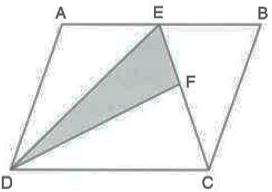
\includegraphics[width=0.4\linewidth]{image.png}
        
    \end{center}
    \begin{options}
        \item 30
        \item 42
        \item 36
        \item 24
    \end{options}
\end{questionbox}



% Задача 28
\begin{questionbox}{28}
    В равнобедренном треугольнике ABC основание AC = 15 и \(\angle BAC = 30^\circ\). Из произвольной точки M на основании AC опущены перпендикуляры на боковые стороны. Найдите сумму длин этих перпендикуляров.
    \begin{options}
        \item 5
        \item \(\frac{15\sqrt{3}}{2}\)
        \item 7,5
        \item 10
    \end{options}
\end{questionbox}



% Задача 29
\begin{questionbox}{29}
    На сторонах AB, BC и CA треугольника ABC взяты точки M, N и P соответственно так, что AM:AB = BN:BC = CP:CA = 1:3. Площадь треугольника MNP равна 2. Найдите площадь треугольника ABC.
    \begin{options}
        \item 7
        \item 5
        \item 4
        \item 6
    \end{options}
\end{questionbox}



% Задача 30
\begin{questionbox}{30}
    Согласно данным на рисунке, найдите градусную меру угла \(\angle DTF = x\).
    \begin{center}
        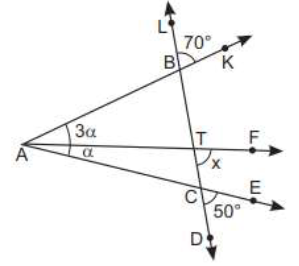
\includegraphics[width=0.5\linewidth]{a.png}
    \end{center}
    \begin{options}
        \item 55
        \item 60
        \item 65
        \item 75
    \end{options}
\end{questionbox}



% Задача 31
\begin{questionbox}{31}
    Согласно данным на рисунке ($AB=AC$), найдите длину отрезка \(|CD| = x\) (в см).
    \begin{center}
         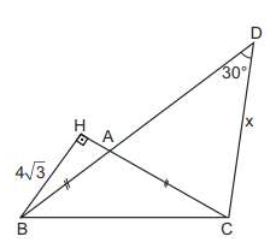
\includegraphics[width=0.4\linewidth]{aa.png}
    \end{center}
    \begin{options}
        \item 8
        \item \(6\sqrt{3}\)
        \item 12
        \item \(8\sqrt{3}\)
    \end{options}
\end{questionbox}



% Задача 32
\begin{questionbox}{32}
В треугольнике ABC угол \(\angle ABC = 50^\circ\) и угол \(\angle ABB = 70^\circ\) . Если AD — высота, а AE — биссектор, найдите угол \(\angle DAE\).
   
   \begin{options}
        \item \(10^\circ\)
        \item \(15^\circ\)
        \item \(20^\circ\)
        \item \(25^\circ\)
    \end{options}
\end{questionbox}



% Задача 33
\begin{questionbox}{33}
   Если в прямоугольной трапеции \(ABCD\)  \(AD=8, \ DC = 6, \ BD = 12\) и \(CE\perp BD\), найдите \(|CE|=x-?\)
    \begin{center}
        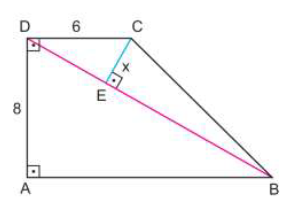
\includegraphics[width=0.5\linewidth]{ddx.png}
    \end{center}
    \begin{options}
        \item \(4\)
        \item \(3\sqrt{2}\)
        \item \(2\sqrt{5}\)
        \item \(2\sqrt{6}\)
    \end{options}
\end{questionbox}






% Задача 34
\begin{questionbox}{34}
    Согласно данным, найдите площадь прямоугольника ABCD (в квадратных единицах). $d: y=\frac{3}{5}x+n$  прямая, B(10,k)
    \begin{center}
       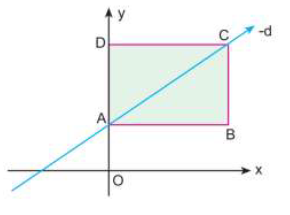
\includegraphics[width=0.5\linewidth]{s.png}
    \end{center}
    \begin{options}
        \item 72
        \item 60
        \item 56
        \item 48
    \end{options}
\end{questionbox}

% Задача 35
\begin{questionbox}{35}
    Если пятизначное число \(\overline{7x142}\) делится на 11 с остатком 2, найдите $x$.
    
    
    \begin{options}
        \item 1
        \item 2
        \item 3
        \item 4
    \end{options}
\end{questionbox}


\end{document}